% ESD descriptor heatmap (supplementary 27-descriptor characterization). Matrix raster: one block per
% scene-phase cell (columns, ordered by the supplementary ESD score) x descriptor (rows);
% value = within-feature percentile rank, as entering the score.
\begin{tikzpicture}[x=1cm,y=1cm,lab/.style={inner sep=0pt,font=\fontsize{7.5}{9}\selectfont}]
\def\mx{5.3}\def\mw{12.4}\def\rh{0.29}
\pgfmathsetmacro\mh{27*\rh}
\node[anchor=north west,inner sep=0pt] at (\mx,0) {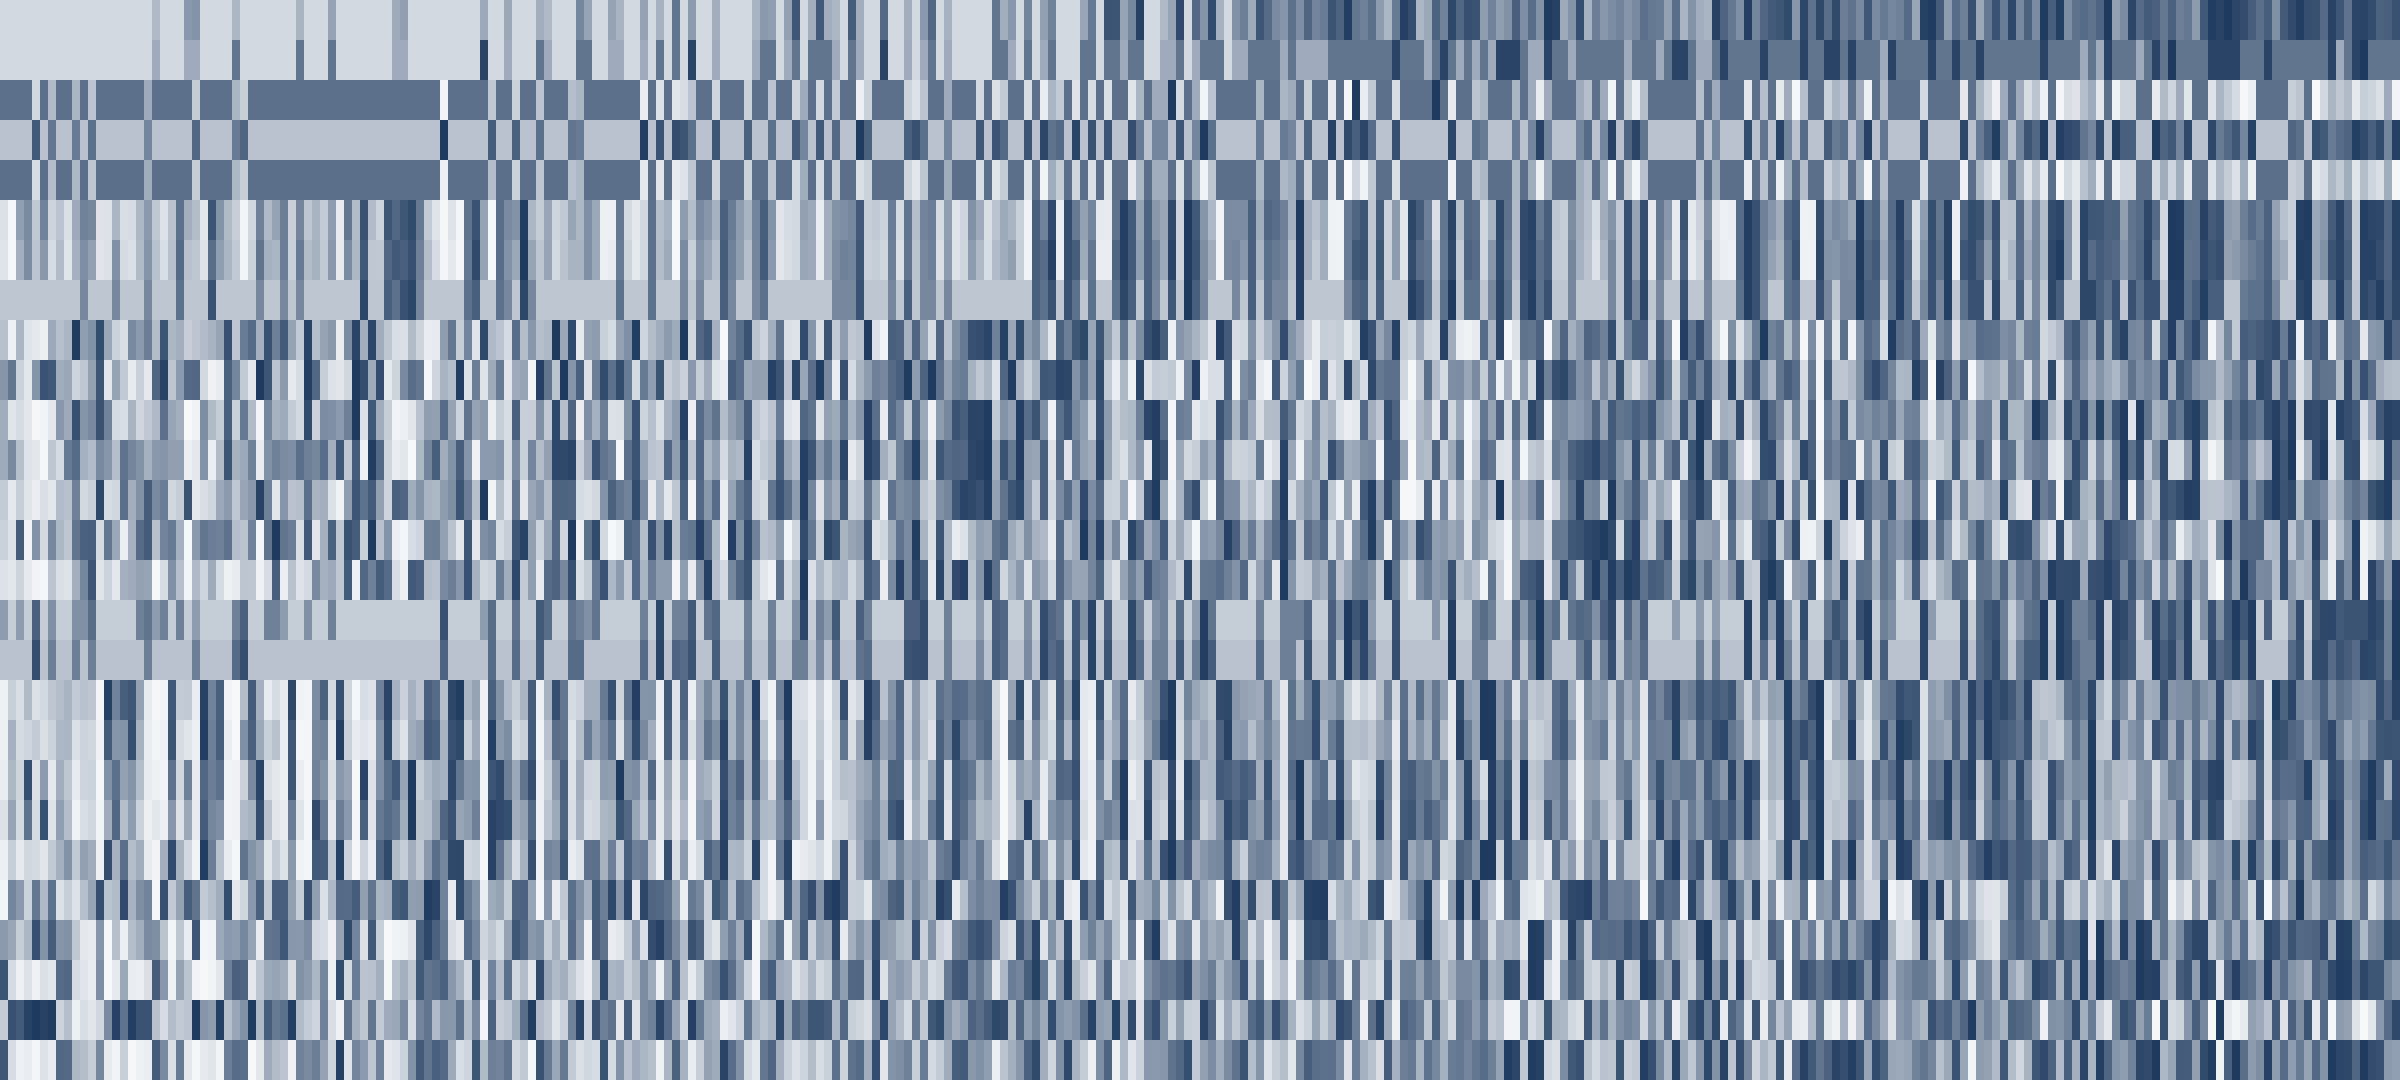
\includegraphics[width=\mw cm,height=\mh cm]{assets/images/appendix/esd_heatmap_27x300.png}};
\draw[rpxAccent,line width=.4pt] (\mx,0) rectangle ++(\mw,-\mh);
\node[lab,anchor=north west,text=rpxInk] at (0,-0.045) {Annotation effort};
\node[lab,anchor=east,font=\fontsize{7.5}{9}\selectfont\ttfamily,text=rpxSlate] at (\mx-.08,-0.145) {iter\_mean};
\node[lab,anchor=east,font=\fontsize{7.5}{9}\selectfont\ttfamily,text=rpxSlate] at (\mx-.08,-0.435) {iter\_max};
\draw[white,line width=1.6pt] (\mx,-0.580) -- ++(\mw,0);
\draw[rpxHair,line width=.3pt] (0,-0.580) -- (\mx-.05,-0.580);
\node[lab,anchor=north west,text=rpxInk] at (0,-0.625) {Scene complexity};
\node[lab,anchor=east,font=\fontsize{7.5}{9}\selectfont\ttfamily,text=rpxSlate] at (\mx-.08,-0.725) {obj\_mean};
\node[lab,anchor=east,font=\fontsize{7.5}{9}\selectfont\ttfamily,text=rpxSlate] at (\mx-.08,-1.015) {obj\_std};
\node[lab,anchor=east,font=\fontsize{7.5}{9}\selectfont\ttfamily,text=rpxSlate] at (\mx-.08,-1.305) {obj\_consist};
\draw[white,line width=1.6pt] (\mx,-1.450) -- ++(\mw,0);
\draw[rpxHair,line width=.3pt] (0,-1.450) -- (\mx-.05,-1.450);
\node[lab,anchor=north west,text=rpxInk] at (0,-1.495) {Occlusion};
\node[lab,anchor=east,font=\fontsize{7.5}{9}\selectfont\ttfamily,text=rpxSlate] at (\mx-.08,-1.595) {occ\_mean};
\node[lab,anchor=east,font=\fontsize{7.5}{9}\selectfont\ttfamily,text=rpxSlate] at (\mx-.08,-1.885) {occ\_p90};
\node[lab,anchor=east,font=\fontsize{7.5}{9}\selectfont\ttfamily,text=rpxSlate] at (\mx-.08,-2.175) {occ\_heavy};
\draw[white,line width=1.6pt] (\mx,-2.320) -- ++(\mw,0);
\draw[rpxHair,line width=.3pt] (0,-2.320) -- (\mx-.05,-2.320);
\node[lab,anchor=north west,text=rpxInk] at (0,-2.365) {Depth quality};
\node[lab,anchor=east,font=\fontsize{7.5}{9}\selectfont\ttfamily,text=rpxSlate] at (\mx-.08,-2.465) {depth\_invalid};
\node[lab,anchor=east,font=\fontsize{7.5}{9}\selectfont\ttfamily,text=rpxSlate] at (\mx-.08,-2.755) {depth\_invalid\_mask};
\node[lab,anchor=east,font=\fontsize{7.5}{9}\selectfont\ttfamily,text=rpxSlate] at (\mx-.08,-3.045) {depth\_std};
\node[lab,anchor=east,font=\fontsize{7.5}{9}\selectfont\ttfamily,text=rpxSlate] at (\mx-.08,-3.335) {depth\_std\_mask};
\draw[white,line width=1.6pt] (\mx,-3.480) -- ++(\mw,0);
\draw[rpxHair,line width=.3pt] (0,-3.480) -- (\mx-.05,-3.480);
\node[lab,anchor=north west,text=rpxInk] at (0,-3.525) {Photometric conflict};
\node[lab,anchor=east,font=\fontsize{7.5}{9}\selectfont\ttfamily,text=rpxSlate] at (\mx-.08,-3.625) {specular};
\node[lab,anchor=east,font=\fontsize{7.5}{9}\selectfont\ttfamily,text=rpxSlate] at (\mx-.08,-3.915) {dark};
\draw[white,line width=1.6pt] (\mx,-4.060) -- ++(\mw,0);
\draw[rpxHair,line width=.3pt] (0,-4.060) -- (\mx-.05,-4.060);
\node[lab,anchor=north west,text=rpxInk] at (0,-4.105) {Temporal stability};
\node[lab,anchor=east,font=\fontsize{7.5}{9}\selectfont\ttfamily,text=rpxSlate] at (\mx-.08,-4.205) {area\_cv};
\node[lab,anchor=east,font=\fontsize{7.5}{9}\selectfont\ttfamily,text=rpxSlate] at (\mx-.08,-4.495) {area\_drop};
\node[lab,anchor=east,font=\fontsize{7.5}{9}\selectfont\ttfamily,text=rpxSlate] at (\mx-.08,-4.785) {vis\_instability};
\draw[white,line width=1.6pt] (\mx,-4.930) -- ++(\mw,0);
\draw[rpxHair,line width=.3pt] (0,-4.930) -- (\mx-.05,-4.930);
\node[lab,anchor=north west,text=rpxInk] at (0,-4.975) {Camera motion};
\node[lab,anchor=east,font=\fontsize{7.5}{9}\selectfont\ttfamily,text=rpxSlate] at (\mx-.08,-5.075) {trans\_mean};
\node[lab,anchor=east,font=\fontsize{7.5}{9}\selectfont\ttfamily,text=rpxSlate] at (\mx-.08,-5.365) {trans\_p90};
\node[lab,anchor=east,font=\fontsize{7.5}{9}\selectfont\ttfamily,text=rpxSlate] at (\mx-.08,-5.655) {rot\_mean};
\node[lab,anchor=east,font=\fontsize{7.5}{9}\selectfont\ttfamily,text=rpxSlate] at (\mx-.08,-5.945) {rot\_p90};
\node[lab,anchor=east,font=\fontsize{7.5}{9}\selectfont\ttfamily,text=rpxSlate] at (\mx-.08,-6.235) {jerk};
\draw[white,line width=1.6pt] (\mx,-6.380) -- ++(\mw,0);
\draw[rpxHair,line width=.3pt] (0,-6.380) -- (\mx-.05,-6.380);
\node[lab,anchor=north west,text=rpxInk] at (0,-6.425) {Fisheye/stereo};
\node[lab,anchor=east,font=\fontsize{7.5}{9}\selectfont\ttfamily,text=rpxSlate] at (\mx-.08,-6.525) {fisheye\_dark};
\node[lab,anchor=east,font=\fontsize{7.5}{9}\selectfont\ttfamily,text=rpxSlate] at (\mx-.08,-6.815) {fisheye\_bright};
\node[lab,anchor=east,font=\fontsize{7.5}{9}\selectfont\ttfamily,text=rpxSlate] at (\mx-.08,-7.105) {fisheye\_sharpness};
\node[lab,anchor=east,font=\fontsize{7.5}{9}\selectfont\ttfamily,text=rpxSlate] at (\mx-.08,-7.395) {fisheye\_corr};
\node[lab,anchor=east,font=\fontsize{7.5}{9}\selectfont\ttfamily,text=rpxSlate] at (\mx-.08,-7.685) {fisheye\_texture};
\draw[rpxInk,line width=.6pt,dash pattern=on 2.2pt off 1.4pt] (\mx+0.3333*\mw,0.95) -- (\mx+0.3333*\mw,-\mh);
\draw[rpxInk,line width=.6pt,dash pattern=on 2.2pt off 1.4pt] (\mx+0.6667*\mw,0.95) -- (\mx+0.6667*\mw,-\mh);
\node[lab,anchor=base,text=tierE] at (\mx+0.1667*\mw,1.02) {Easy (100)};
\node[lab,anchor=base,text=tierM] at (\mx+0.5000*\mw,1.02) {Medium (100)};
\node[lab,anchor=base,text=tierH] at (\mx+0.8333*\mw,1.02) {Hard (100)};
% ESD characterization score of each column
\begin{scope}[shift={(\mx,0.12)},x=\mw cm,y=0.68cm]
  \draw[rpxHair,line width=.3pt] (0,0) rectangle (1,1);
  \draw[rpxAccent,line width=.6pt] plot coordinates {(0.0050,0.0250) (0.0150,0.0468) (0.0250,0.1169) (0.0350,0.1325) (0.0450,0.1484) (0.0550,0.1703) (0.0650,0.1809) (0.0750,0.1853) (0.0850,0.1907) (0.0950,0.2084) (0.1050,0.2245) (0.1150,0.2322) (0.1250,0.2370) (0.1350,0.2420) (0.1450,0.2607) (0.1550,0.2718) (0.1650,0.2832) (0.1750,0.2904) (0.1850,0.2952) (0.1950,0.3051) (0.2050,0.3088) (0.2150,0.3106) (0.2250,0.3153) (0.2350,0.3237) (0.2450,0.3271) (0.2550,0.3292) (0.2650,0.3326) (0.2750,0.3367) (0.2850,0.3437) (0.2950,0.3451) (0.3050,0.3493) (0.3150,0.3555) (0.3250,0.3622) (0.3350,0.3694) (0.3450,0.3895) (0.3550,0.3978) (0.3650,0.4026) (0.3750,0.4137) (0.3850,0.4166) (0.3950,0.4237) (0.4050,0.4279) (0.4150,0.4317) (0.4250,0.4375) (0.4350,0.4471) (0.4450,0.4553) (0.4550,0.4734) (0.4650,0.4814) (0.4750,0.4864) (0.4850,0.4908) (0.4950,0.4980) (0.5050,0.4990) (0.5150,0.5091) (0.5250,0.5191) (0.5350,0.5254) (0.5450,0.5379) (0.5550,0.5419) (0.5650,0.5527) (0.5750,0.5576) (0.5850,0.5654) (0.5950,0.5704) (0.6050,0.5768) (0.6150,0.5851) (0.6250,0.5920) (0.6350,0.6004) (0.6450,0.6016) (0.6550,0.6055) (0.6650,0.6145) (0.6750,0.6221) (0.6850,0.6236) (0.6950,0.6258) (0.7050,0.6274) (0.7150,0.6356) (0.7250,0.6426) (0.7350,0.6517) (0.7450,0.6642) (0.7550,0.6782) (0.7650,0.6804) (0.7750,0.6851) (0.7850,0.6901) (0.7950,0.6911) (0.8050,0.6921) (0.8150,0.6946) (0.8250,0.7066) (0.8350,0.7129) (0.8450,0.7141) (0.8550,0.7216) (0.8650,0.7272) (0.8750,0.7415) (0.8850,0.7468) (0.8950,0.7547) (0.9050,0.7580) (0.9150,0.7755) (0.9250,0.7782) (0.9350,0.7868) (0.9450,0.7955) (0.9550,0.8035) (0.9650,0.8176) (0.9750,0.8523) (0.9850,0.8683) (0.9950,0.9129)};
\end{scope}
\node[lab,anchor=east,text=rpxSlate] at (\mx-.08,.46) {ESD score};
\node[lab,anchor=north west,text=rpxSlate] at (\mx,-\mh-.12) {300 scene--phase cells, ordered by ESD characterization score $\rightarrow$};
% colour key
\shade[left color={rgb,255:red,247;green,249;blue,251},right color={rgb,255:red,30;green,58;blue,95}] (\mx+\mw-4.05,-\mh-.2) rectangle ++(1.9,-.22);
\draw[rpxAccent,line width=.3pt] (\mx+\mw-4.05,-\mh-.2) rectangle ++(1.9,-.22);
\node[lab,anchor=east,text=rpxSlate] at (\mx+\mw-4.13,-\mh-.31) {0};
\node[lab,anchor=west,text=rpxSlate] at (\mx+\mw-2.07,-\mh-.31) {1\enspace percentile rank};
\end{tikzpicture}
